\chapter{研究基础与相关技术}

近年来,深度学习一直是计算机领域乃至多学科交叉应用领域的研究热点,不仅在计算机视觉方向有着广泛的应用,在光学、材料和航空航天等领域也出现了相关研究。尤其对于大数据应用场景,基于深度学习的方法已经成为重要的数据挖掘手段。
对于气动优化乃至整个CFD领域而言,深度学习方法在此领域获得发展并取得成功只是时间问题。
为了便于阐述本课题工作,本章首先定义了本课题要解决的问题,即明确利用深度学习方法和技术要解决的问题和要达到的效果;
其次介绍了CFD相关的基础理论,主要包括建立在宏观层次的Navier-Stokes(N-S)方程和介观层次的格子Boltzmann方法(Lattice Boltzmann Methods,LBM);最后介绍了本文涉及到的深度学习相关的技术和方法,包括基于深度神经网络(Deep Neural Networks,DNN)和图神经网络(Graph  Neural Networks,GNN)的网络架构等。

\section{研究问题定义}
利用传统CFD方法对流体问题(包括气动优化问题)进行研究的流程如图\ref{fig:cfdflow}所示。
\begin{figure}[htp]
	\centering
	%\includegraphics[width=0.42\textwidth]{data/MLP.pdf}
	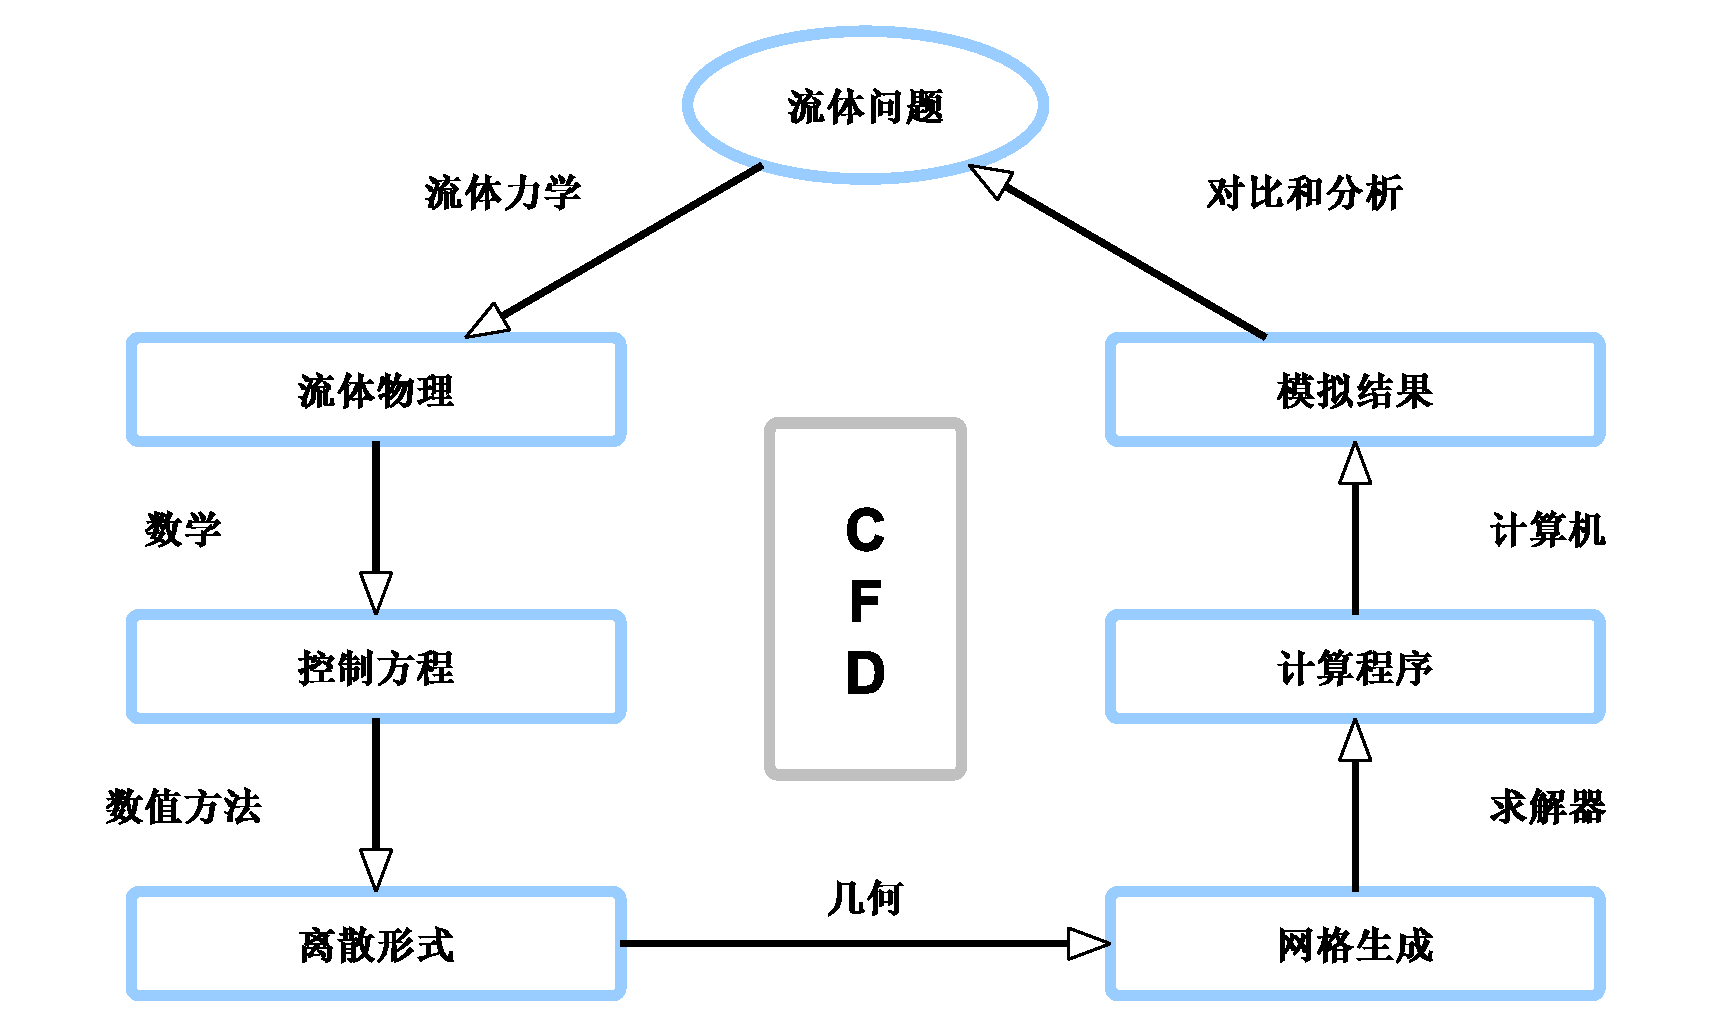
\includegraphics[width=0.92\textwidth]{figures/cfdflow.pdf}
	\caption{利用传统CFD方法研究和解决流体问题的流程示意图}
	\label{fig:cfdflow}
\end{figure}


首先利用流体力学知识对流体问题进行理论分析,建立物理模型;
根据流体运动遵循的基本规律,利用数学方法推导出流体流动的控制方程,
宏观层面上有粘性流动的Navier-Stokes方程和无粘流动的欧拉方程;
针对特定的流体问题,明确其物理基础和假设,简化控制方程、确定边界条件和初始条件。
由于CFD方法是利用数值计算对流体流动进行模拟,所以研究的不是连续运动的流体,必须利用数值方法对时间和空间进行离散,
以便进行迭代计算求解。对空间的离散方法包括有限差分方法,有限元方法和有限体积方法;
对时间的离散通常包括适用于定常流体问题求解的显示方法和适用于非定常问题的求解的隐式方法。
确定离散形式之后,需要对几何进行划分,即生成网络,在网格上对控制方程进行求解。
网格生成之后,选择合适的CFD求解器,依据初始条件和边界条件对求解器的参数进行设置,
最后利用计算机进行迭代计算至模拟结果收敛。



这种全阶CFD模拟往往耗时较长,难以满足全面、快速的设计空间探索需求。
为了加速CFD模拟进程,提升气动优化效率,本文针对二维稳态流动问题,
提出了两种基于深度学习的气动优化模型,图\ref{fig:cfd_dnnflow}展示了这两种模型的工作流程。

\begin{figure}[htp]
	\centering
	%\includegraphics[width=0.42\textwidth]{data/MLP.pdf}
	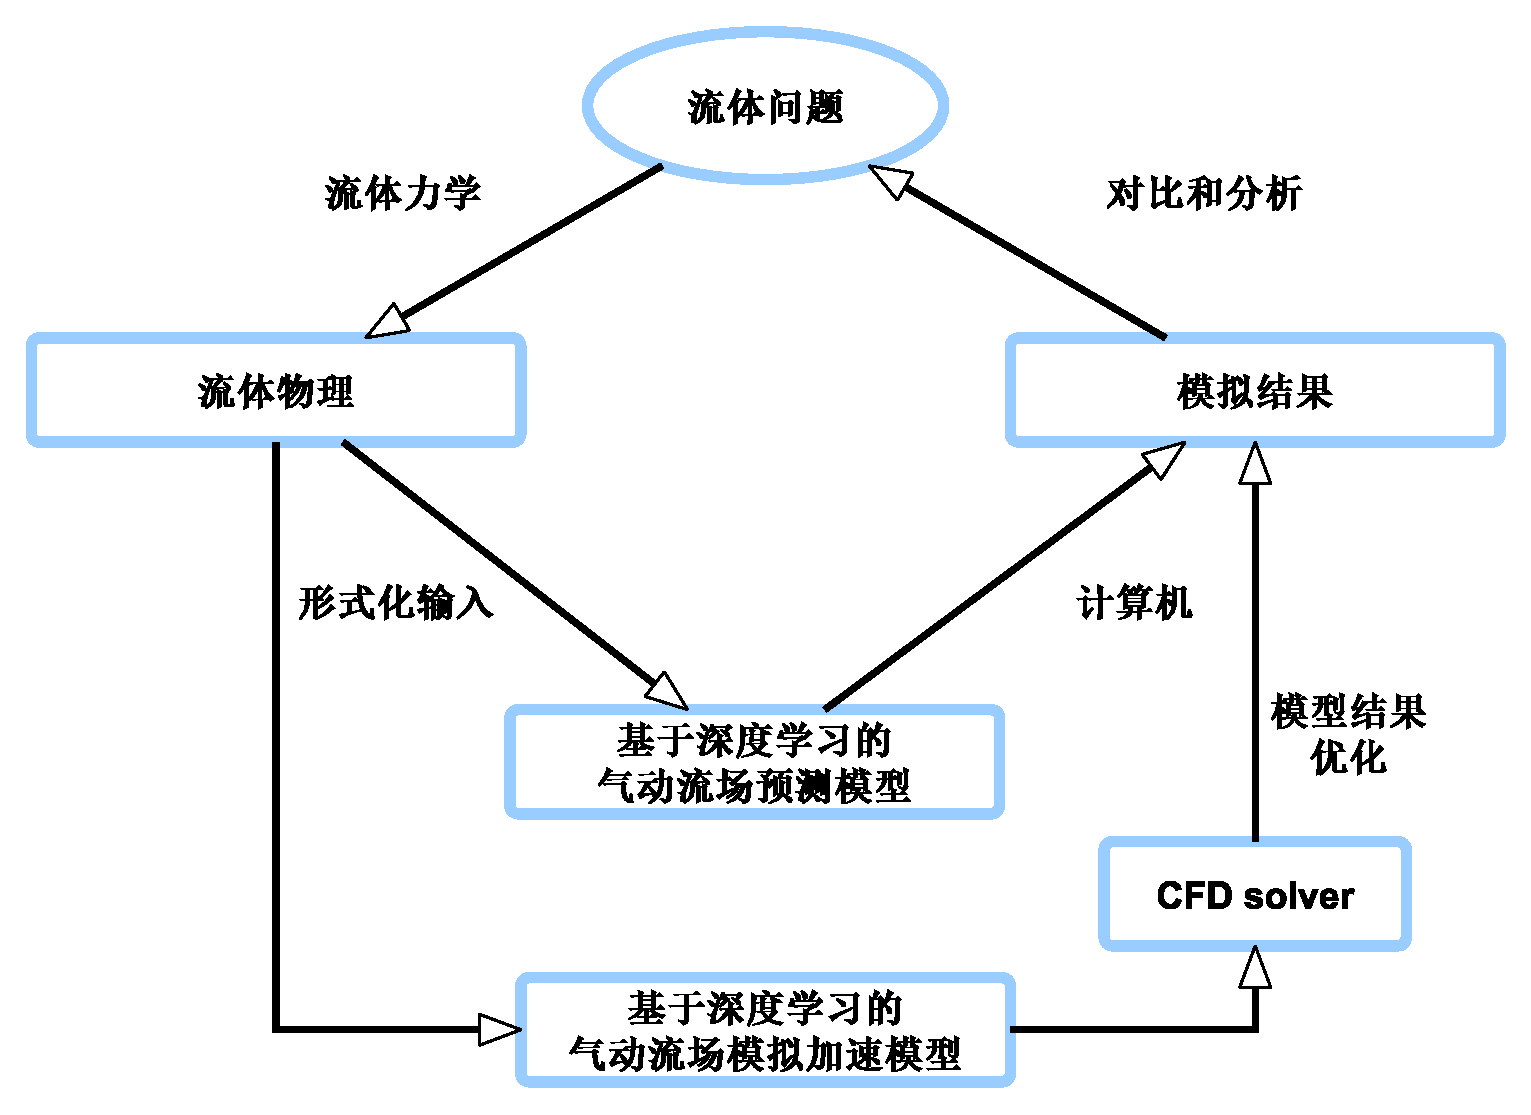
\includegraphics[width=0.92\textwidth]{figures/cfd_dnnflow.pdf}
	\caption{基于深度学习的气动优化模型工作流程示意图}
	\label{fig:cfd_dnnflow}
\end{figure}

在气动流场预测模型中,将边界条件和几何外形形式化为适合神经网络训练的输入,
利用深度学习方法构建端到端的预测模型,通过神经网络正向推理过程,得到对应的气动流场预测结果;
气动流场模拟加速模型的流程与气动流场预测模型类似,不同之处在于模型训练完成后,将深度学习模型的结果输入到CFD求解器中,为CFD求解过程提供一个更加接近收敛状态的初场,从而达到减少迭代计算量、加速模拟的效果。



\section{计算流体动力学基础理论}
根据对气体在不同尺度上动力学规律的描述,计算流体力学方法可分为三类:宏观、介观和微观。

宏观尺度上,假设流体连续地充满整个空间,流体被假设为连续介质。满足质量守恒、动量守恒以及能量守恒;在数学上,流体可由欧拉方程组、N-S方程组进行描述;在数值计算上,通过各种离散方法将欧拉方程组或N-S方程组离散成各种代数方程。
介观尺度(分子自由程尺度)上,流体被离散为一系列流体粒子;在数学上,流体由统计力学方程描述;在数值计算上,构造符合一定物理规律的演化机制,通过演化得到与物理规律相符的数值结果。
微观尺度上,不再假设流体介质为连续的,通过对每一个分子的运动进行模拟计算,
然后在采用不同的方式进行统计平均,以获得流体的宏观运动规律。因为要对每一个分子的运动进行模拟计算,微观层面的方法往往需要消耗大量的计算资源。
根据与本文研究内容的相关性,本节重点介绍格子Boltzmann方法和雷诺平均N-S方程。



\subsection{格子Boltzmann方法的基本原理}

\subsubsection{BGK模型}
Boltzmann方程的基本思想是
在任何一个宏观系统中,每一个分子的微观运动都遵循力学规律,因此只要算出大量分子的个别运动就可以确定系统的宏观参数;
求出每一分子处于某种状态下的概率,通过统计的方法得出系统的宏观参数。 
基于以上思想,物理学家 Boltzmann提出方程的三大假设:
\begin{itemize}
	\item[(1)] 分子相互碰撞只考虑二体碰撞,认为3个及3个以上分子碰撞的概率很小;
	\item[(2)] 各个分子的速度分布是不依赖于另外的分子而独立存在;
	\item[(3)] 外力不影响局部碰撞的动力学行为。 	
\end{itemize}

定义速度分布函数$f$是空间位置矢量$\vec{r}$,分子速度矢量$\vec{\xi}$以及时间$t$的函数。根据$f$的定义有:
\begin{equation}n=\int f(\vec{r}, \vec{\xi}, t) d \xi\end{equation}
\noindent n即为t时刻,$\vec{r}$处单位体积内的分子数。
根据假设,速度分布函数$f$可由两项引起改变,第一项是分子的运动,第二项是分子的碰撞,
先考虑没有碰撞的情况,$m \vec{a}$为作用在每个分子上的外力,m是分子质量,
任意分子,如果在时间间隔$d t$内无碰撞,则分子位置由$\vec{r}$变为$\vec{r}+d \vec{r}$,
速度变为$\vec{\xi}+\vec{a} d t$,则原t时刻,在$d \vec{r} d \vec{\xi}$中的气体分子全部转移到$\vec{r}+d \vec{r}$,$\vec{\xi}+\vec{a} d t$的$d \vec{r} d \vec{\xi}$中,即有
\begin{equation}f(\vec{r}+d \vec{r}, \vec{\xi}+\vec{a} d t, t+d t) d \vec{r} d \vec{\xi}=f(\vec{r}, \vec{\xi}, t) d \vec{r} d \vec{\xi}\end{equation}

\noindent 在$(\vec{r}, \vec{\xi}, t)$处进行Taylor展开,化简有分子的运动对速度分布函数f的影响:

\begin{equation}
\label{运动}
\left(\frac{\partial f}{\partial t}\right)_{\text {运动 }}=-\vec{\xi} \cdot \frac{\partial f}{\partial \vec{r}}-\vec{a} \cdot \frac{\partial f}{\partial \vec{\xi}}\end{equation}

\noindent 考虑分子间的碰撞,应用刚体碰撞模型,根据碰撞前后动量守恒和能量守恒可得碰撞对速度分布函数的影响:

\begin{equation}
\label{碰撞}
\left(\frac{\partial f_{1}}{\partial t}\right)_{\text {碰撞 }}=\iint\left(f_{1}^{\prime} f_{2}^{\prime}-f_{1} f_{2}\right) d_{D}^{2}|\vec{g}| \cos \theta d \Omega d \vec{\xi}_{2}\end{equation}

\noindent  其中$\vec{g} =  f_{1} - f_{2}$, $f_{1}$,$f_{2}$为碰撞前分子速度,$f_{1}^{\prime}$,$f_{2}^{\prime}$是碰撞后分子速度;$d_{D}$是分子直径,
$d \Omega$表示球面微元在第一个分子的固定角。

综合公式\ref{运动}和\ref{碰撞}有:
\begin{equation}\left(\frac{\partial f}{\partial t}\right)=\left(\frac{\partial f}{\partial t}\right)_{\text {运动 }}+\left(\frac{\partial f}{\partial t}\right)_{\text {碰撞 }}\end{equation}

\noindent 化简即有:
\begin{equation}
\label{Boltzmann方程}
\left(\frac{\partial f}{\partial t}\right)+\vec{\xi} \cdot \frac{\partial f}{\partial \vec{r}}+\vec{a} \cdot \frac{\partial f}{\partial \vec{\xi}}=\iint\left(f_{1}^{\prime} f_{2}^{\prime}-f_{1} f_{2}\right) d_{D}^{2}|\vec{g}| \cos \theta d \Omega d \vec{\xi}_{1}\end{equation}

由于碰撞项计算涉及复杂的非线性积分,所以Boltzmann方程难以求解。因此,Bhatnagar,Gross和Krook提出使用一个简单的算子$\Omega_{f}$替代方程\ref{Boltzmann方程}右边碰撞项,称为BGK近似模型。
最简单的算子可以认为碰撞使f趋于平衡分布$f^{e q}$。设改变率与$\left(f^{e q}-f\right)$成正比,系数为$\nu$,为碰撞频率即弛豫时间的导数${1}/{\tau_{0}}$,则Boltzmann方程简化为:

\begin{equation}\left(\frac{\partial f}{\partial t}\right)+\vec{\xi} \cdot \frac{\partial f}{\partial \vec{r}}+\vec{a} \cdot \frac{\partial f}{\partial \vec{\xi}}=v\left[f^{e q}(\vec{r}, \vec{\xi}, t)-f(\vec{r}, \vec{\xi}, t)\right]\end{equation}

\noindent 等式右边即为线性算子$\Omega_{f}$。

\subsubsection{格子Boltzmann方程}
格子Boltzmann方程是BGK方程的进一步离散形式,这一离散形式包括了速度离散、时间离散、空间离散。
对于时间离散,由于微观粒子时刻在做无规则的热运动,因此微观粒子的速度是连续的,其速度方向和大小有无穷个,但粒子的运动并不会显著影响流体的宏观运动。
因此可以将分子速度简化为有限维速度空间,$\left\{\overrightarrow{e_{0}}, \vec{e}_{1}, \ldots, \overrightarrow{e_{N}}\right\}$,N表示速度种类数。
连续的速度分布函数f也被相应离散为$\left\{f_{0}, f_{1}, \ldots, f_{N}\right\}$,
其中$f_{\alpha}=f_{\alpha}\left(\vec{r}, \overrightarrow{e_{\alpha}}, t\right)$,
$\alpha=0,1, \ldots, N$。于是可得离散的Boltzmann方程:

\begin{equation}
\label{速度离散}
\frac{\partial f_{\alpha}}{\partial t}+\overrightarrow{e_{\alpha}} \cdot \nabla f_{\alpha}=-\frac{1}{\tau_{0}}\left(f_{\alpha}-f_{\alpha}^{e q}\right)+F_{\alpha}\end{equation}

\noindent 其中$f_{\alpha}^{e q}$分子局部平衡分布;$F_{\alpha}$为离散速度空间的外力项。
在速度离散的基础上,进一步进行时间离散和空间离散,对公式\ref{速度离散}积分,采用矩形法对公式右边项进行逼近有:

\begin{equation}
\label{LBM方程}
f_{\alpha}\left(\vec{r}+\overrightarrow{e_{\alpha}} \delta_{t}, t+\delta_{t}\right)-f_{\alpha}(\vec{r}, t)=-\frac{1}{\tau}\left[f_{\alpha}(\vec{r}, t)-f_{\alpha}^{e q}(\vec{r}, t)\right]+\delta_{t} F_{\alpha}(\vec{r}, t)\end{equation}

方程\ref{LBM方程}即为格子Boltzmann方程。
DnQm模型\cite{Y1992Lattice}是格子Boltzmann方程基本模型,n表示空间维数,m表示速度的类型,常见的有D2Q7模型、D2Q9模型、D3Q15模型和D3Q19模型等,图\ref{fig:dnqm}给出了D2Q9和D3Q19的示意图。


\begin{figure}[htb]
	\centering
	\subfloat[D2Q9]{\label{fig:d2q9}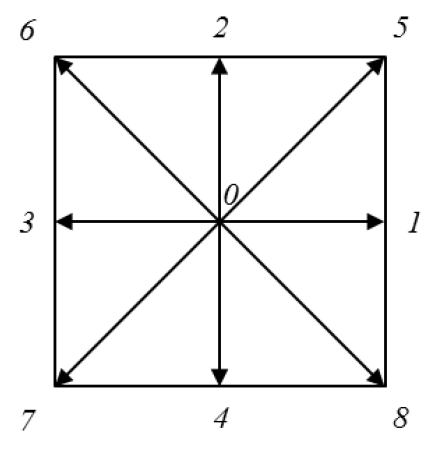
\includegraphics[width=0.35\textwidth]{figures/d2q9.png}} \qquad
	\subfloat[D3Q19]{\label{fig:d3q19}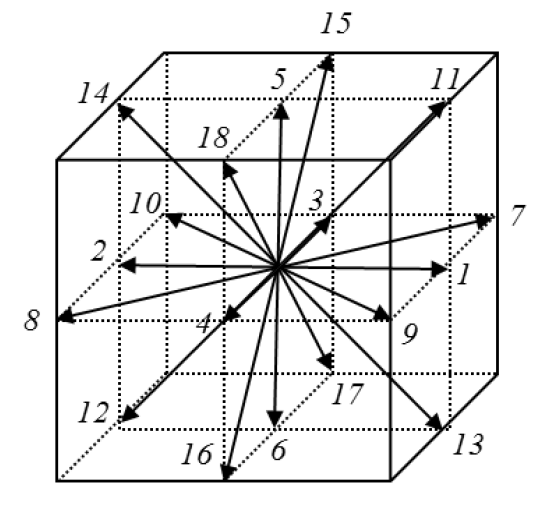
\includegraphics[width=0.38\textwidth]{figures/d3q19.png}} 
	\caption{D2Q9模型和D3Q19模型速度离散示意图}
	\label{fig:dnqm}
\end{figure}

\noindent D2Q9模型适用于二维流动问题,将速度根据大小和方向的不同分为了9类;
D3Q19模型适用于三维流动问题,速度离散也更加复杂,将速度根据大小和方向的不同分为了19类。

LBM方法相对于宏观方法具有精度高的特点,与传统方法相比,对流项(碰撞项)是线性的,算法简单;由于粒子的运动只有碰撞和迁移,LBM方法编程容易;
此外,LBM运算具有局部性,每个粒子只与周围相邻粒子有关,局部运算可同步进行,适合并行计算。
因为以上优点,LBM方法在CFD领域应用广泛,利用深度学习技术提升LBM方法的模拟效率具有重要意义。


\subsection{雷诺平均N-S(RANS)方程}
流体流动一般由以下三个基本定律来控制:
(1)质量守恒定律;(2)牛顿第二定律;(3)能量守恒定律。基于这三个基本的物理学定理构建的流动模型,将导出一组控制方程,比如适合粘性流动的Navier-Stokes方程(N-S方程)。

流体流动有不同的流动状态,当流速很小时,流体分层流动,互不混合,称为层流;当流速逐渐增大,流体的流线开始出现波浪状的摆动,摆动的频率及振幅随流速的增加而增加,此种流况称为过渡流;当流速增加到很大时,流线不再清楚可辨,流场中有许多小漩涡,层流被破坏,相邻流层间出现滑动和混合,这时的流体作不规则运动,这种运动称为湍流。

湍流运动过程十分复杂,在数学上表现出极高的非线性,使用数值模拟方法解决湍流一直是流体力学研究的难点。
虽然N-S方程能够准确地描述湍流运动的细节,但求解这样一个复杂的方程会花费大量的精力和时间。

目前在CFD领域,解决湍流问题的方法主要包括直接数值模拟(Direct numerical simulation,
DNS)、大涡模拟(Large eddy simulation,LES)和雷诺平均( Reynold average Navier-Stokes,RANS)。
其中DNS和LES对网格精细度要求较高,在工程应用上还处于尚不成熟的阶段。
为了在精度和效率上满足实际工程需要,研究者提出了基于时均理论的雷诺平均N-S模型,RANS在工程上应用也最多。
对于本文研究的稳态不可压流动,在笛卡尔坐标系下有,连续性方程:

\begin{equation}
\label{连续性方程}
\frac{\partial \rho}{\partial t}+\frac{\partial(\rho u)}{\partial x}+\frac{\partial(\rho v)}{\partial y}+\frac{\partial(\rho w)}{\partial z}=0\end{equation}

\noindent 对动量方程采用二阶迎风对流格式离散:


\begin{equation}\begin{array}{c}
\label{动量方程}
u \frac{\partial u}{\partial x}+v \frac{\partial u}{\partial y}+w \frac{\partial u}{\partial z}=-\frac{1}{\rho} \frac{\partial p}{\partial x}+\frac{\mu}{\rho} \nabla^{2} u \\
u \frac{\partial v}{\partial x}+v \frac{\partial v}{\partial y}+w \frac{\partial v}{\partial z}=-\frac{1}{\rho} \frac{\partial p}{\partial y}+\frac{\mu}{\rho} \nabla^{2} v \\
u \frac{\partial v}{\partial x}+v \frac{\partial w}{\partial y}+w \frac{\partial w}{\partial z}=-\frac{1}{\rho} \frac{\partial p}{\partial z}+\frac{\mu}{\rho} \nabla^{2} w
\end{array}
\end{equation}


\noindent 对方程\ref{连续性方程}和\ref{动量方程}进行雷诺平均有:
\begin{equation}\frac{\partial \rho}{\partial t}+\frac{\partial}{\partial x_{i}}\left(\rho \bar{u}_{i}\right)=0\end{equation}

\begin{equation}\frac{\partial}{\partial t}\left(\rho \bar{u}_{i}\right)+\frac{\partial}{\partial x_{i}}\left(\rho \bar{u}_{j} \bar{u}_{i}\right)=-\frac{\partial \bar{p}}{\partial x_{i}}+\frac{\partial \bar{\sigma}_{i j}}{\partial x_{j}}+\frac{\partial}{\partial x_{j}}\left(-\rho \bar{u}_{i}^{\prime} \bar{u}_{j}^{\prime}\right)\end{equation}

\noindent 其中$\bar{u}_{i}$为雷诺平均速度分量,$\rho$为密度,$p$为压强,$\bar{u}_{i}^{\prime}$平均脉动速度,$\partial \bar{\sigma}_{i j}$为应力张量分量。


一般地,在对湍流流动的N-S方程平均后,得到的平均方程中会包含未知的雷诺应力项,导致了方程求解的不封闭问题。
因此需要根据湍流运动规律以寻找附加条件和关系式构建湍流模型使方程封闭。
此外,在进行雷诺平均的过程中损失了部分流动细节,引入湍流模型对于找回这些细节十分必要。
对于RANS湍流模拟,根据Boussinesq\cite{schmitt2007boussinesq}假设,粘性系数由层流部分和湍流部分构成,
即$\nu=\nu_{L}+\nu_{T}$,其中$\nu_{L}$是层流运动粘性系数(laminar kinematic viscosity), $\nu_{T}$是湍流运动粘性系数(eddy-viscosity variable),由湍流模型方程计算得到。

常用的湍流模型可根据所采用的微分方程数进行分类为:零方程模型、一方程模型、两方程模型、四方程模型、七方程模型等\cite{1998A}。本文使用的湍流模型是Spalart-Allmaras(SA)模型\cite{SAequation},
是一种主要用在航空领域的单方程湍流模型,对墙壁束缚(wall-bounded)流动,显示出很好的效果。
SA模型认为在自由剪切流中能量和信息由大尺度流动流向小尺度流动,涡粘系数只有产生项和扩散项,所以满足以下基本运输方程:

\begin{equation}
\begin{split}
\frac{D F}{D t}= & \frac{\partial F}{\partial t}+(u \cdot \nabla) F \\ = & {Diffusion} + {Production} - {Destruction}
\end{split}
\end{equation}

\noindent 其中$F$外力,\textit{diffusion}是扩散项,\textit{production}是产生项,\textit{destruction}是损失项。
对于湍流运动粘性系数$\nu_{T}$应用该运输方程有:

\begin{equation}\label{SA_equo}
\begin{split}
\frac{D \nu_{T}}{D t}=& \frac{1}{\sigma}\left[\nabla \cdot((\nu_{L}+\nu_{T}) \nabla \nu_{T})+c_{b 2}(\nabla \nu_{T})^{2}\right] +c_{b 1} \tilde{S} \nu_{T} - \\ &c_{w 1} f_{w}\left[\frac{\nu_{T}}{d}\right]^{2}
\end{split}
\end{equation}

\noindent 其中$\sigma$普朗特数,$c_{b 1}$和$c_{b 2}$为闭合常数,$d$表示到壁面的最短距离。
$\tilde{S}$可以通过$d$和速度$u$计算得到,
$f_{w}$是一个关于$\tilde{S}$和$\nu_{T}$无量纲函数,用于解决在边界层外部损失项收敛慢的问题。

虽然许多湍流模型在某些特定的应用场景取得成功,但至今仍未有一个有效的通用的湍流模型,这也直接导致了RANS缺少普适性。

\FIXME{本文就是要通过DL模拟求解器中复杂的迭代运算}


\section{深度学习相关模型介绍}
深度学习是机器学习的重要分支,自2006年提出以来,深度学习理论和技术以及获得了长足的发展,常见的深度学习模型有深度信念网络\cite{深度信念网络},自动编码器\cite{Bengio2013Representation},卷积神经网络\cite{Lecun1998Gradient},递归神经网络\cite{Williams2014A},生成对抗网络\cite{GAN}等。
此外,深度学习在与强化学习、图网络结合方面也非常成功,比较前沿的研究领域有深度强化学习\cite{Deepreinforcementlearning}和图神经网络\cite{2016Semi}等。
深度学习的快速发展为解决气动优化提供了新的思路和方法,
利用深度学习方法提升气动优化效率的核心思想是基于神经网络构建从输入到输出的映射函数,
从而代替或者加速CFD求解器的迭代计算过程,
不同于常规的图像分类任务,深度神经网络需要在大量数据中学习到从给定输入到对应输出的表示方法。

针对流场数据中的欧式空间数据,经过类比分析,我们发现图像处理中的image-to-image\cite{DBLP:conf/miccai/RonnebergerFB15,DBLP:conf/cvpr/LongSD15,isola2017image,CycleGAN2017,DBLP:conf/cvpr/AmodioK19}的转换方法尤其适用于气动优化场景。
对于非欧式空间数据,本文引入了基于图神经网络的架构进行模型训练。
如何将流场数据处理成为深度神经网络可接受的形式将在第三章详细阐述,本节重点介绍三类用于图像回归任务的深度神经网络和图神经网络。
关于深度学习的其他基础理论知识,包括网络基础结构单元,损失函数,优化算法等,可参见文献\cite{dnnsurvey}。

\subsection{卷积自编码网络}
卷积自编码网络(Convolutional Autoencoders)是自编码网络\cite{Bengio2013Representation}的变体。
自编码网络及其变体都有类似的网络结构:编码器和解码器。
传统的自编码器是一种无监督学习算法,数据没有标签,
输入数据$X$经过编码器处理得到输入数据的特征表示z,编码结果经过解码器得到输出$X^{\prime}$,具体过程可以表示为:
\begin{equation}
z=g(X ; \phi) 
\vspace{-0.2cm}
\end{equation}
\begin{equation}
X^{\prime}=f(z ; \theta)
\end{equation}
其中$g(\bullet ; \phi)$和$f(\bullet ; \theta)$分别表示编码器和解码器,$\phi$和$\theta$是相应的参数。

损失函数一般可以定义为输入$X$和输出$X^{\prime}$的最小均方误差(Mean Squared Error,MSE):
\begin{equation}
Loss_{MSE} = \min _{\phi, \theta}\left\|X-X^{\prime}\right\|_{2}^{2}
\end{equation}

一般而言,z的维度远小于输入$X$的维度,网络通过这样编码和解码的方式,实现对输入数据的降维且尽量不损失数据信息。

但是传统的自编码器在处理图片格式数据时,由于采用了全连接操作,忽略了图像中的空间关系,数据切片和数据堆叠会导致信息大量丢失。
为了克服这一缺点,卷积自编码网络采用卷积层来构造自编码器。
图\ref{fig:CAE}是卷积自编码网络的示意图,深色部分代表编码器,通常由卷积层和池化层构成,卷积层负责信息提取,池化层负责空域下采样;
浅色部分代表解码器,由卷积层和上采样层构成,有时也利用逆卷积操作替代卷积和上采样操作进行原始信息的复原。

\begin{figure}[htp]
	\centering
	%\includegraphics[width=0.42\textwidth]{data/MLP.pdf}
	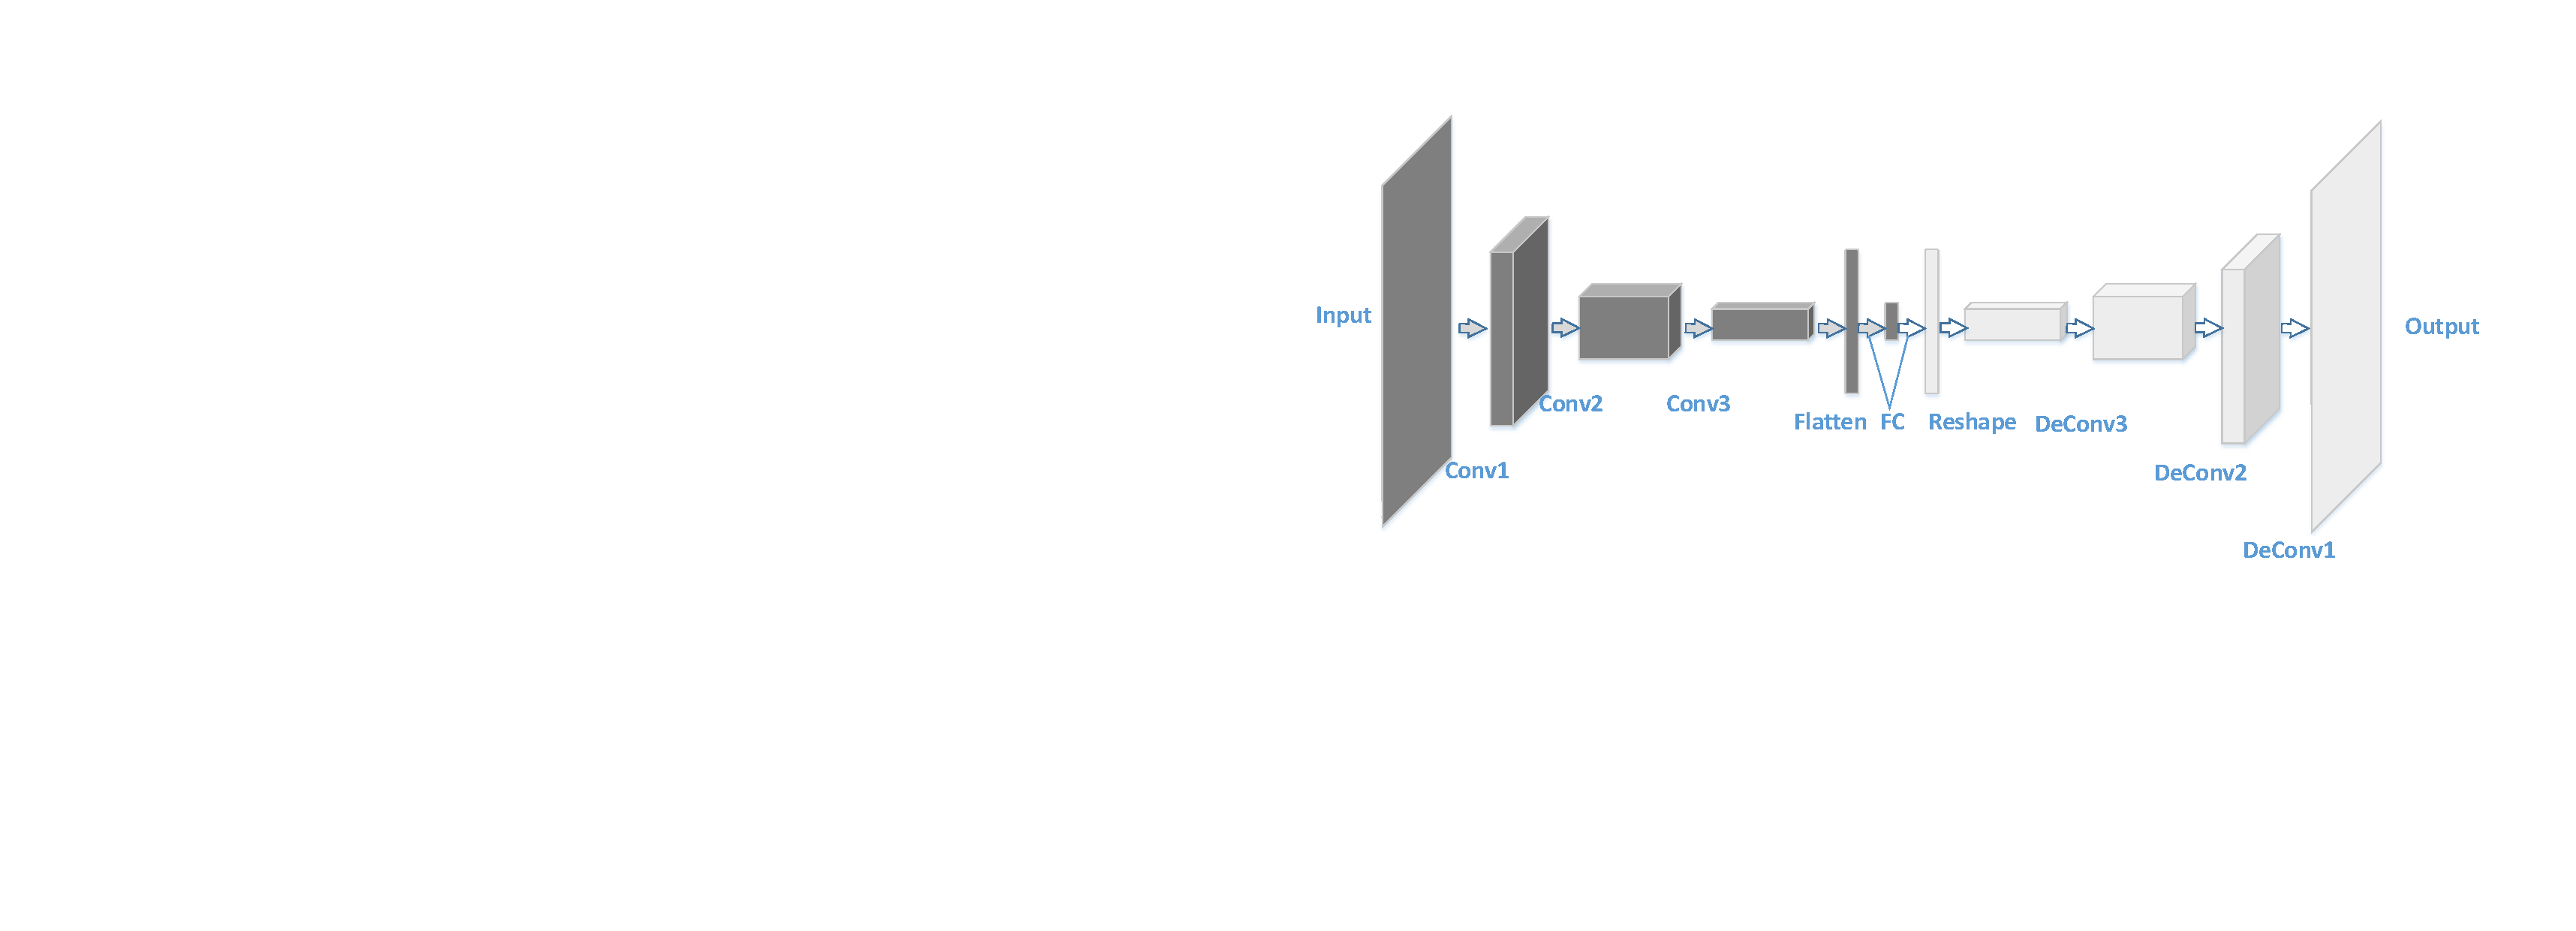
\includegraphics[width=0.92\textwidth]{figures/CAE.pdf}
	\caption{卷积自编码网络示意图}
	\label{fig:CAE}
\end{figure}

逆卷积操作原理如图\ref{fig:conv_dconv}所示,逆卷积操作可以看出是常规卷积操作的逆过程,不同点在于,为了还原原始输入的尺寸,通常需要进行填充(padding)操作(如图\ref{fig:dconv}中的空白区域)。


\begin{figure}[htb]
	\centering
	\subfloat[卷积操作]{\label{fig:conv}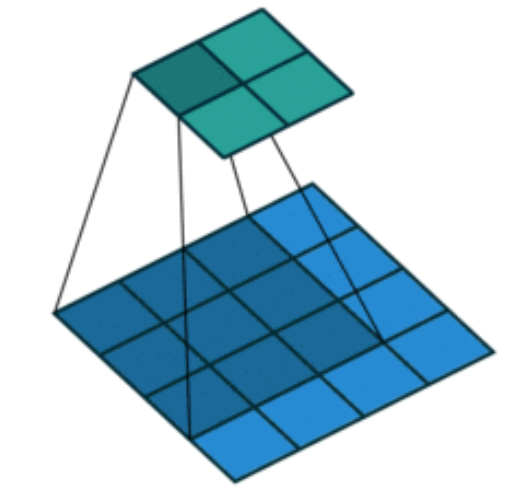
\includegraphics[width=0.42\textwidth]{figures/conv.png}} \qquad
	\subfloat[逆卷积操作]{\label{fig:dconv}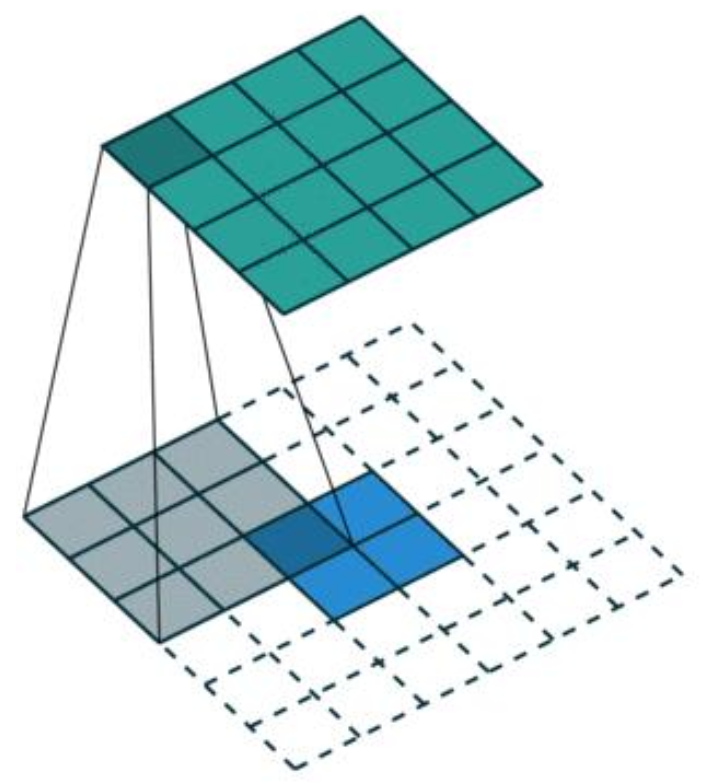
\includegraphics[width=0.38\textwidth]{figures/dconv.png}} 
	\caption{逆卷积操作原理}
	\label{fig:conv_dconv}
\end{figure}

%\begin{figure}[htp]
%	\centering
%	%\includegraphics[width=0.42\textwidth]{data/MLP.pdf}
%	subfigure[卷积操作]{\label{fig:conv}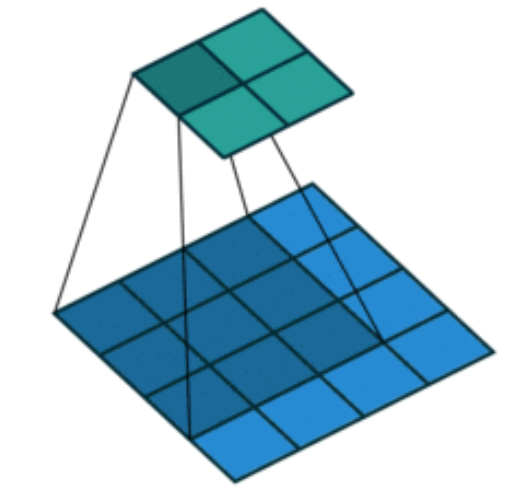
\includegraphics[width=0.42\textwidth]{figures/conv.png}}
%	subfigure[逆卷积操作]{\label{fig:dconv}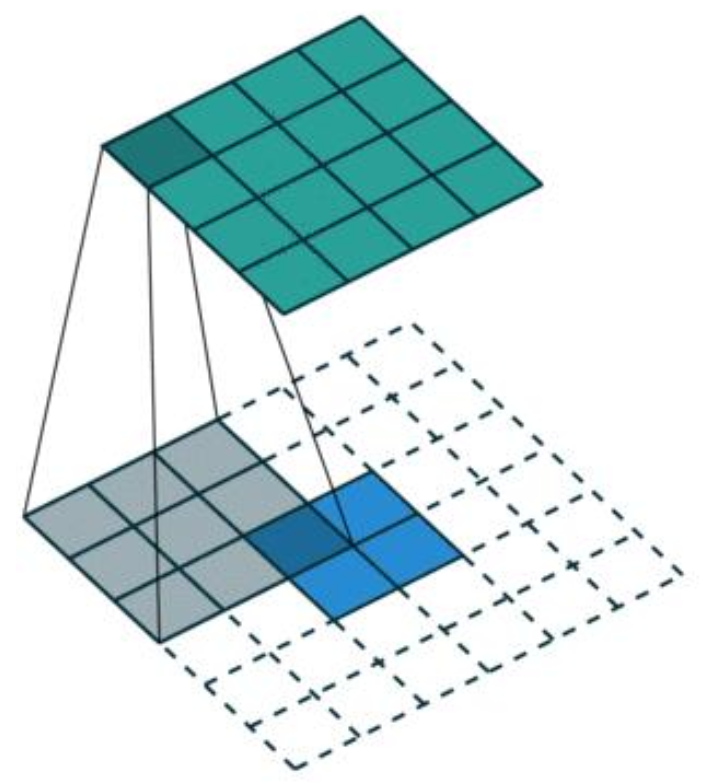
\includegraphics[width=0.42\textwidth]{figures/dconv.png}}
%	\caption{逆卷积操作原理}
%	\label{fig:conv_dconv}
%\end{figure}


对于无监督学习,在卷积神经网络的编码器和解码器的衔接处,利用全连接层,也可以提取带图像数据特征表示;在进行有监督学习时,网络更关注解码器的输出$Y^{\prime}$而不是z,损失函数转化为:
\begin{equation}
Loss_{MSE} = \min _{\phi, \theta}\left\|Y-Y^{\prime}\right\|_{2}^{2}
\end{equation}
从而可以利用卷积神经网络进行有监督学习任务,在气动流场模拟领域已有基于卷积自编码网络开展的工作\cite{DBLP:conf/kdd/GuoLI16}。



\subsection{基于深度学习的图像分割模型}
图像分割一直是计算机视觉领域的难题,也是该领域的研究热点。
所谓图像分割是指根据灰度、彩色、空间纹理、几何形状等特征把图像划分成若干个互不相交的区域,使得这些特征在同一区域内表现出一致性或相似性,而在不同区域间表现出明显的不同。
传统的方法有基于阈值的分割方法;基于区域的图像分割方法;基于边缘检测的分割方法;基于小波分析和小波变换的分割方法;基于遗传算法的分割方法等\cite{图像分割方法综述}。

近年来,深度学习方法开始应用到图像分割,通过搭建神经网络,对训练样本进行有监督学习,得到图形分割的模型。根据分割应用任务不同,图像分割分可分为普通分割、语义分割和实例分割。其中:普通分割是指对分属不同区域的像素点进行分类;语义分割是在分类的基础上识别出每一块区域的语义;实例分割在在语义分割的基础上,进一步对每个识别目标进行编号。本节重点介两种经典的语义分割网络:全卷积网络和U-net网络,分别适用于自然图像分割和医疗图像分割。


\subsubsection{全卷积网络}
2015年Long等人提出的全卷积网络(Fully Convolutional Networks,FCN)用于图像语义分割\cite{Long2015Fully}。自从提出后,FCN已经成为语义分割的基本框架,后续算法都借鉴了该框架的思想。

\begin{figure}[htp]
	\centering
	%\includegraphics[width=0.42\textwidth]{data/MLP.pdf}
	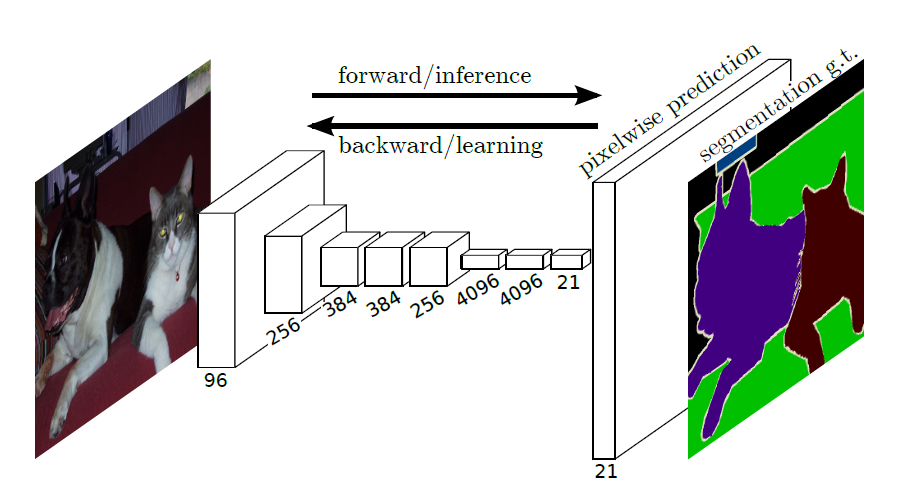
\includegraphics[width=0.88\textwidth]{figures/FCN.png}
	\caption{FCN网络结构图}
	\label{fig:FCN}
\end{figure}

如图\ref{fig:FCN}所示,FCN参考了图像分类网络中的VGG16\cite{2014Very}网络架构。图像分类网络只能对整个图片进行分类而不能识别每个像素点的类别。
为了实现逐像素分类的目的,FCN用卷积层替换了VGG网络中的全连接层,最后利用逆卷积的上采样方法将特征图恢复成原始图片大小,从对整张图片的稀疏分类转换成对每个像素点进行密集分类(dense prediction),达到图像分割的目的。

FCN的另一个特点是利用了全局信息和局部信息。经过多次卷积和池化操作以后,得到的图像越来越小,分辨率越来越低,最后产生了高维特征图。如果直接对进行上采样至原始图片大小,会产生模糊的分割结果。为了解决这一问题,FCN使用了如图\ref{fig:FCN_skip}所示的skip layer的方法。

对于FCN-32s,高层得到的粗糙层(conv7)进行32倍上采样操作,再对每个点进行softmax逻辑回归处理,得到每一个像素点的分类。

对于FCN-16s,先将conv7的结果进行2倍上采样,再将上采样结果与浅层的精细层(pool4)进行逐点相加,最后进行16倍的上采样操作得到与原始输入尺寸相同的图像分割结果。

对于FCN-8s,先将conv7的结果进行4倍上采样,将pool4的结果进行2倍上采样,再将上采样结果与更浅层的精细层(pool3)进行逐点相加,最后进行8倍上采样操作和softmax处理。

通过skip layer的方法,融合多层特征图,有效整合了粗粒度的语义信息和细粒度的位置信息,有利于提高分割准确性。
尽管8倍上采样的FCN的分割效果已经有了很大提升,但是结果还是比较模糊,对分割区域边界不敏感;此外,对每个像素点单独进行分类,没有充分考虑图像的空间上的联系。

\begin{figure}[htp]
	\centering
	%\includegraphics[width=0.42\textwidth]{data/MLP.pdf}
	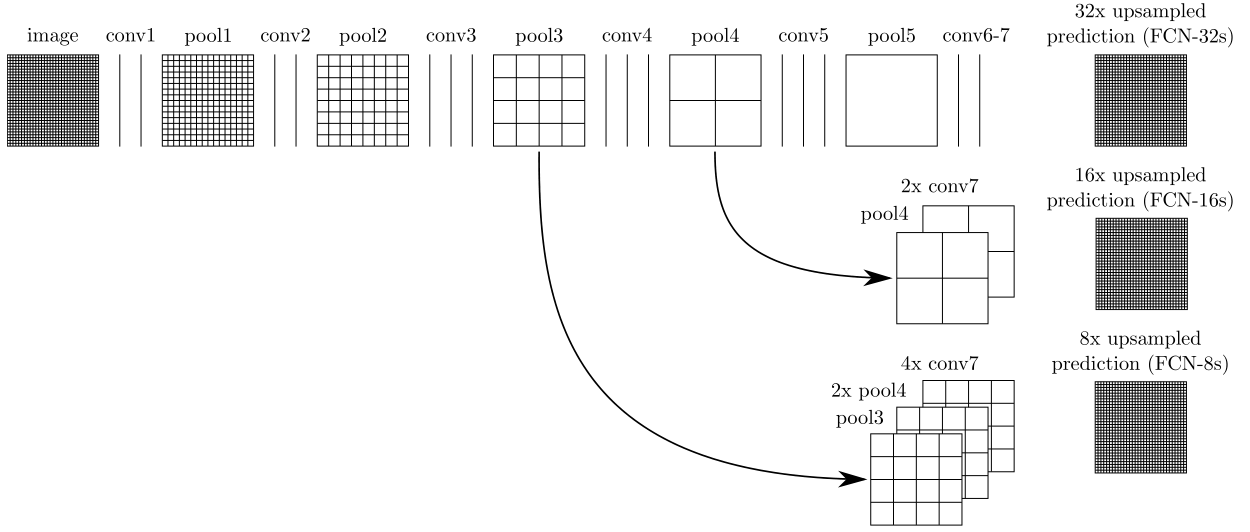
\includegraphics[width=0.88\textwidth]{figures/FCN_skip.png}
	\caption{FCN采用的skip layer方法}
	\label{fig:FCN_skip}
\end{figure}

\subsubsection{U-net网络}
2015年,Ronneberger等人\cite{DBLP:conf/miccai/RonnebergerFB15}提出了U-net网络结构,U-net是基于FCN的一种语义分割网络,适用于做医学图像的分割。U-net修改并扩展了FCN网络结构,使它在使用少量的数据进行训练的情况下获得精确的分割结果。
其主要思想是在下采样网络的后面补充一个对称的上采样网络,多个上采样层增加了网络的参数和表示能力,有利于提升输出结果的分辨率。
对称的网络结构形似英文字母“U”,所以被称为U-net。

U-net网络结构如图\ref{fig:unet}所示:
蓝/白色框表示特征图;蓝色箭头表示3x3卷积层,用于特征提取;灰色箭头表示 skip-connection,用于特征融合;红色箭头表示池化层,用于降低维度;绿色箭头表示上采样 upsample,用于恢复维度;青色箭头表示1x1卷积,用于输出结果。其中灰色箭头中的copy就是atenate操作,将深层的特征图和浅层的特征图在通道方向拼接;crop是为了让两者的长宽一致,保证拼接后的特征图大小一致。


\begin{figure}[htp]
	\centering
	%\includegraphics[width=0.42\textwidth]{data/MLP.pdf}
	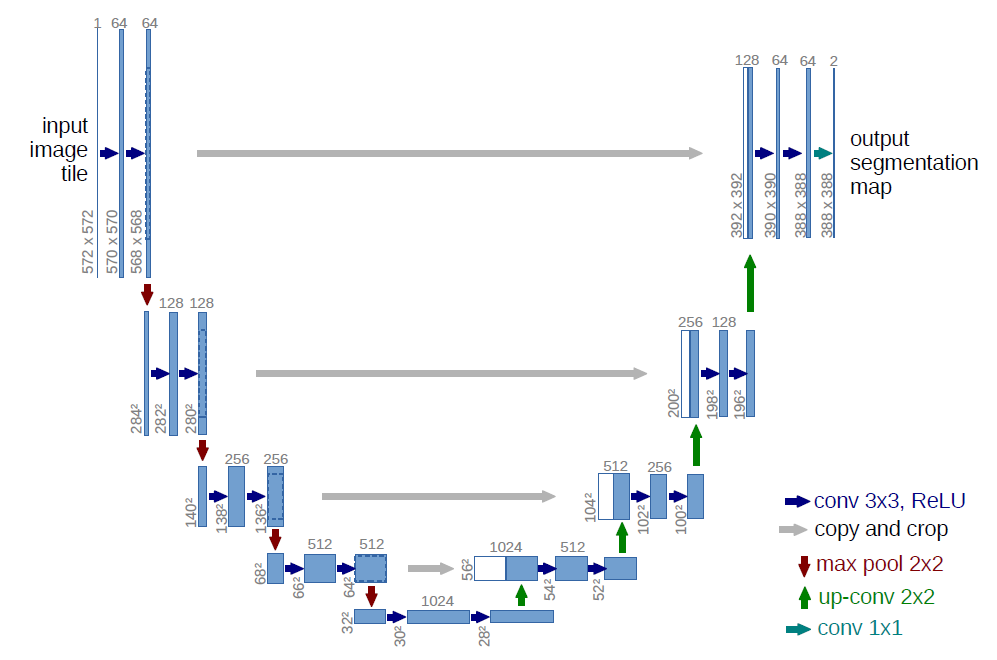
\includegraphics[width=0.88\textwidth]{figures/unet.png}
	\caption{U-net网络结构图\cite{DBLP:conf/miccai/RonnebergerFB15}}
	\label{fig:unet}
\end{figure}

U-net主体结构包括一个捕获上下文信息的收缩路径和一个允许精确定位的对称拓展路径:
收缩部分和扩展部分都有4个采样层。这种架构延续了Encoder-Decoder的思想。
Encoder由卷积操作和下采样操作组成,文中所用的卷积结构统一为3x3的卷积核,填充为 0,步长为1;Decoder部分采用的上采样的方式与FCN中的反卷积不同,为双线性插值。
此外,为了更好融合位置信息和语义信息,U-net拓展了FCN中skip layer的思想,在“U”形网络的对称部分添加了skip connection。与FCN的加操作不同,U-net使用了叠操作(concatenation)增加了特征的厚度,保留了更多浅层的位置信息,这使得上采样层可以在浅层特征与深层特征在训练时进行自适应选择,这对语义分割任务来说更有优势。

由于在医疗图像分割上取得巨大成功,许多研究者针对不同的图像分割任务对U-net进行了改进,产生了许多U-net变体包括V-Net\cite{2016V}、UNet++\cite{unet++}、U-NetPlus\cite{unetplus}和3D U2-Net\cite{20193D}等,提升了模型的推理速度和精度。


\subsection{Pix2Pix网络模型}
对于气动流场预测,核心问题是实现从输入到输出的映射。
除了前文提到的自编码网络和图像分割网络,基于生成对抗网络(Generative Adversarial Network, GAN)的图像风格迁移模型也在解决像素到像素的映射问题上展示出的强大潜力。
GAN在图像生成、风格迁移、超分辨重建等领域已经得到了广泛的应用,
本节我们重点介绍Pix2Pix网络模型\cite{isola2017image}。

Pix2Pix网络基于条件生成对抗网络(Conditional Generative Adversarial Network, cGAN)\cite{cGAN},通过添加条件约束信息来指导完成图像转换任务,比如从标签图合成相片,从线稿图重构对象,给图片上色等。
和传统的GAN网络类似,在Pix2Pix模型训练过程中,迭代地训练生成器和判别器,生成器尽可能生成接近真实的样本,企图“欺骗”判别器;判别器尽可能识别出真实的样本和生成的样本,获得更高的得分。这样的对抗训练过程类似博弈游戏,随着训练的进行,生成器和判别器的能力不断提升直到达到令人满意的效果。
由于添加了约束条件,Pix2Pix网络的输入不再是普通GAN网络中的随机变量,其网络结构示意图
如图\ref{fig:cgan}所示:

\begin{figure}[htp]
	\centering
	%\includegraphics[width=0.42\textwidth]{data/MLP.pdf}
	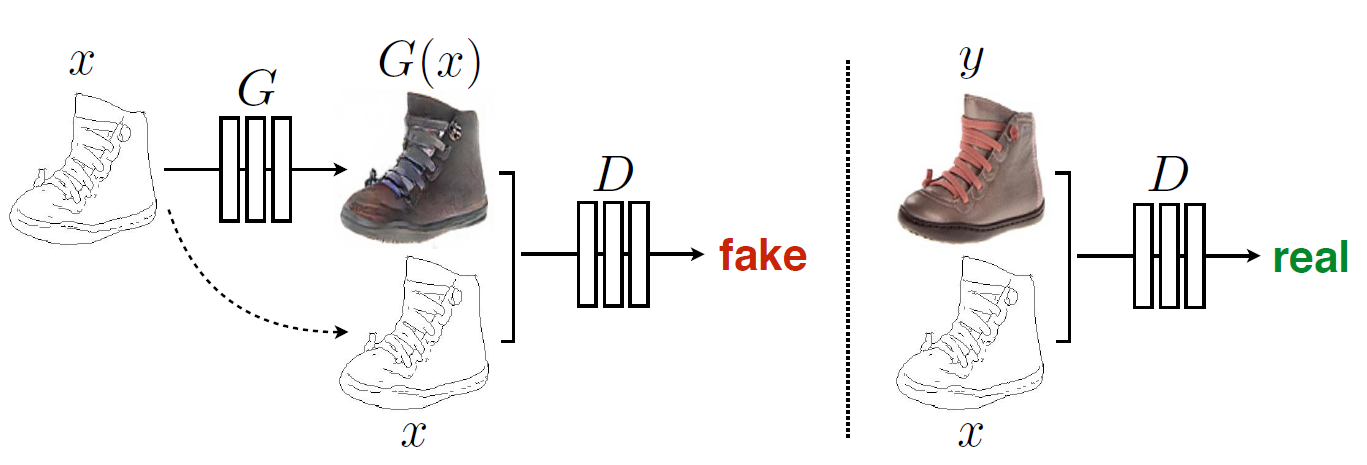
\includegraphics[width=0.88\textwidth]{figures/cGAN.png}
	\caption{Pix2Pix网络结构示意图}
	\label{fig:cgan}
\end{figure}

其中x是条件输入,y是对应的标签,每个输入x唯一对应一个标签y。
在训练生成器时,x进过生成器$G$得到生成图像$G(x)$;
在训练判别器时,输入x和对应生成图像$G(x)$或标签y通过通道维度的叠操作进行拼接,一同送入判别器,判别器会输出概率值,表示是否为一对真实样本。



Pix2Pix网络利用类似U-net的结构代替自编码网络作为生成器,
在输入和输出之间存在很多可以共享的低级信息,采用skip-connection的结构有利于传递这些底层信息和重构图像。
对于判别器网络,Pix2Pix提出了PatchGAN架构。
传统GAN判别器通常对生成样本整体进行判断,对于图片而言,直接输出整张图片是真实样本的概率。而图像转换任务中关注像素到像素的转换效果,所以在这里提出了分块判断的算法,在图像的每个块上去判断是否为真,输出平均预测结果。


条件GAN采用的损失函数通常为:
\begin{equation}
\begin{aligned}
\mathcal{L}_{c G A N}(G, D)= &\mathbb{E}_{x,y}[\log D(x,y)]+\\
&\mathbb{E}_{x,z }[\log (1-D(x, G(x,z))]
\end{aligned}
\end{equation}

\begin{equation}
\begin{aligned}
\mathcal{L}_{c G A N}(G)= \mathbb{E}_{x,z}[\log (1-D(x, G(x, z))]
\end{aligned}
\end{equation}

\noindent 其中z为输入随机变量,在Pix2Pix网络输入仅为x。
此外,为了保证像素级低频信息的预测精度,Pix2Pix网络的损失函数还引入了$L_1$损失项:

\begin{equation}
\begin{aligned}
\mathcal{L}_{L 1}(G)=\mathbb{E}_{x_1, x_2, y}\left[\|y-G(x_1, x_2)\|_{1}\right]
\end{aligned}
\end{equation}

考虑到训练的最终目标是获得一个性能良好的生成器,同时生成器和判别器进行着对抗的训练,所以训练的最终目标是:
\begin{equation}
\begin{aligned}
G^{*}=\arg \min _{G} \max _{D} \mathcal{L}_{c G A N}(G, D)+\lambda \mathcal{L}_{L 1}(G)
\end{aligned}
\end{equation}
\noindent 其中$\lambda$是$L_1$损失函数项的权重系数。


\subsection{图卷积神经网络}

在深度学习发展过程中,卷积神经网络(Convolutional Neural Network, CNN)和循环神经网络(Recurrent Neural Network, RNN)在图像识别、语义分割、自然语言处理等领域发挥了重要作用。
无论是图像还是语言,在CNN或RNN进行处理时都被转换成结构规则的数据形式,都属于欧式空间的数据。
然而现实生活中有很多不规则的数据结构,如社交网络、化学分子结构、生物网络等;即使是语言,其内部实际是复杂的树形结构,
只是RNN将其处理成向量的形式便于神经网络训练。
图结构通常被用来表示这些非欧式空间的数据,但是在图结构中,每个节点周围的结构千差万别,不同于图像和向量化的语言数据具有平移不变性,因此不可能直接利用CNN或RNN进行处理。

近年来,人们对深度学习方法在图上的拓展进行了大量的研究,研究人员借鉴CNN、RNN以及图嵌入技术的思想,
定义和设计了专用于处理图结构数据的神经网络,即图神经网络(Graph  Neural  Network, GNN)。
文献\cite{2019A}将GNN分为五大类:图卷积网络(Graph Convolution Networks,GCN)、 图注意力网络(Graph Attention Networks)、图自编码器( Graph Autoencoders)、图生成网络( Graph Generative Networks) 和图时空网络(Graph Spatial-temporal Networks)。
本节重点介绍图卷积神经网络\cite{2016Semi}。

和卷积神经网络类似,GCN可以使用多层神经网络对图数据进行特征提取,层与层之间的传播方式如下:

\begin{equation}
H^{(l+1)}=\sigma\left(\tilde{D}^{-\frac{1}{2}} \tilde{A} \tilde{D}^{-\frac{1}{2}} H^{(l)} W^{(l)}\right)
\end{equation}

\noindent 其中$H^{(l)} \in R^{N \times d^{(l)}}$是第$l$层图结构特征表达,维度是$N \times d^{(l)}$,
$N$表示图节点数目,$d^{(l)}$是节点特征维度。
矩阵$\tilde{A} = A + I$,其中A是图节点的邻接矩阵,I是单位矩阵,
表示每个节点在下一层状态不仅与自己的邻居有关还与节点本身有关。
矩阵$\tilde{D}$是$\tilde{A}$的度矩阵,用于归一化处理;
$W^{(l)}$是权重矩阵,在图卷积网络训练过程中不断调整;$\sigma$代表非线性激活函数。

\begin{figure}[htp]
	\centering
	%\includegraphics[width=0.42\textwidth]{data/MLP.pdf}
	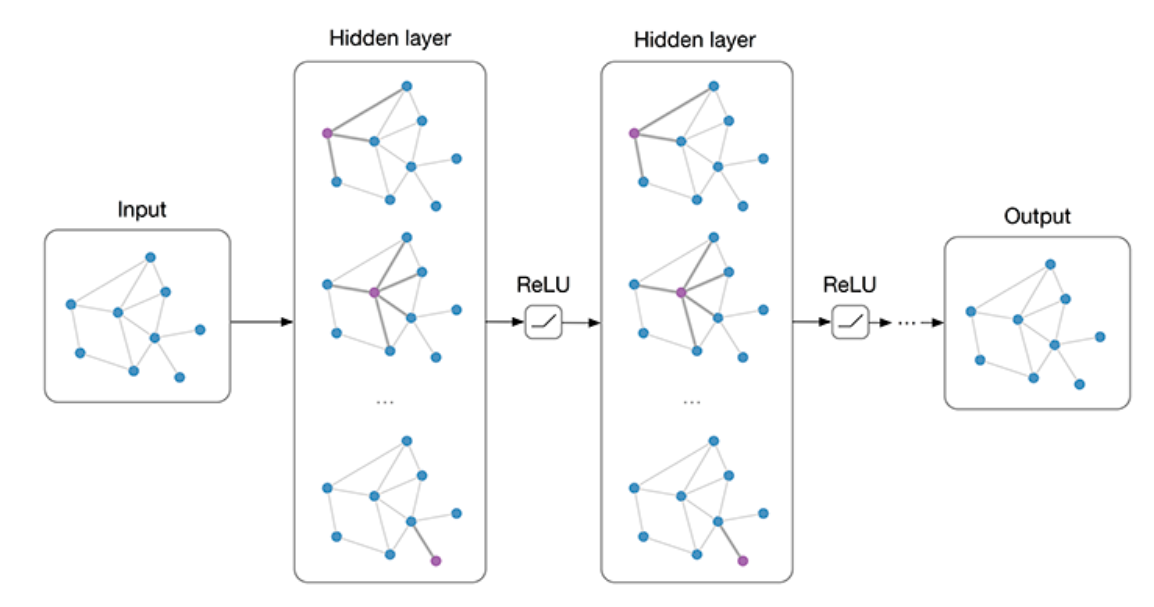
\includegraphics[width=0.88\textwidth]{figures/GCN.png}
	\caption{多层GCN网络示意图}
	\label{fig:gcn}
\end{figure}

对于图卷积算法的实现主要包括三个步骤:
\romannumeral1)发送:每一个节点将自身的特征信息经过变换后发送给邻居节点。这一步是在对节点的特征信息进行抽取变换;
\romannumeral2)接收:每个节点将邻居节点的特征信息聚集起来。这一步是在对节点的局部结构信息进行融合;
\romannumeral3)变换:把前面的信息聚集之后做非线性变换,增加模型的表达能力。
图\ref{fig:gcn}展示了一个简单的GCN网络,从图中可以发现数据的拓扑结构在训练过程中始终保持不变,
所以图卷积算子中$\tilde{D}^{-\frac{1}{2}} \tilde{A} \tilde{D}^{-\frac{1}{2}}$可以在训练之前确定并在训练中重复利用。
每一层的节点特征维度是不固定的,可以根据训练任务的复杂程度进行灵活的调整。

概括而言,图卷积算子的作用就是将每个节点的特征与其邻居节点的特征加权平均后传播到下一层,具有以下特点:
1)局部参数共享,计算节点特征值时,按一定规律将参与聚合的节点分为若干个子集,
同一个子集内的节点采用相同的权重;
2)节点感受域正比于层数,每一层图卷积运算只能和相邻的节点进行特征聚合;通过增加GCN层数,每个节点上参与运算的其他节点信息就更多;
3)适用于任意拓扑结构的节点与图,能同时对节点特征信息与结构信息进行端对端学习,是目前对图数据学习任务的最佳选择。




\section{实验算例介绍}


\subsection{2D不可压层流固体外部流场}


\subsection{2D不可压有粘翼型外部流场}




\section{本章小结}
